\section{Fish biomass response to El Nino conditions}

This section describes the fish biomass response to El Nino conditions and analyses the underlying mechanisms. The focus will be laid on the three strongest El Nino events on records, 1982, 1997 and 2015 \citep{santosoDefiningCharacteristicsENSO2017}. The 1982 and 1997 events are Eastern Pacific El Ninos, whose ocean response has been extensively described and analyzed in terms of physics  (e.g. \citealt{mcphadenGenesisEvolution1997981999, vialardModelStudyOceanic2001, lengaigneOceanResponseMarch2002}), biogeochemistry \citep{chavezBiologicalChemicalResponse1999, gierachBiologicalResponse19972012} and ecosystems \citep{leaObservationsFishesAssociated2000, glynnCoralBleachingMortality2001,arcosJackMackerelFishery2001}. On the other hand, the 2015 event is a combination of Central Pacific/Eastern Pacific conditions, with warmer subsurface and surface temperature anomalies in the west-central Pacific and cooler ones in the eastern Pacific \citep{lheureuxObservingPredicting20152017}. 

In order to capture the generic fish biomass response to extreme El Nino events, independently to the intrinsic characteritics of each event, composite analysis has been performed by averaging temperature, ocean velocity, LTL concentrations and fish biomass anomalies over the 1982, 1997 and 2015 years.

\subsection{El Nino fish biomass anomalies}

Left column of Fig\ref{fig:mean_ond97_ape} shows the October, November and December composites of fish biomass density anomalies (colors), to which the climatological mean is superimposed (black contours). On average, fish biomass for small epipelagics is maximal at around 5\degree{}N and 5\degree{}S (see the $2.0$ contour on Fig \ref{fig:mean_ond97_ape}a), while smaller biomass is found at the equator and in the eastern Pacific. During El Nino conditions, biomass anomalies superimposes over the mean states, which may indicate an equatorward and an eastward shift of biomass location.
As size increases, the location of the biomass minimum on the central eastern Pacific extends westward and poleward, while the positive anomalies associated with El Nino conditions follow the same pattern: for intermediate sizes (Fig\ref{fig:mean_ond97_ape}b), the positive anomalies reach 180\degree{}E, while for small sizes, the anomalies are located east of 150\degree{}W. 

\begin{figure}[h!tp]
	\centering
	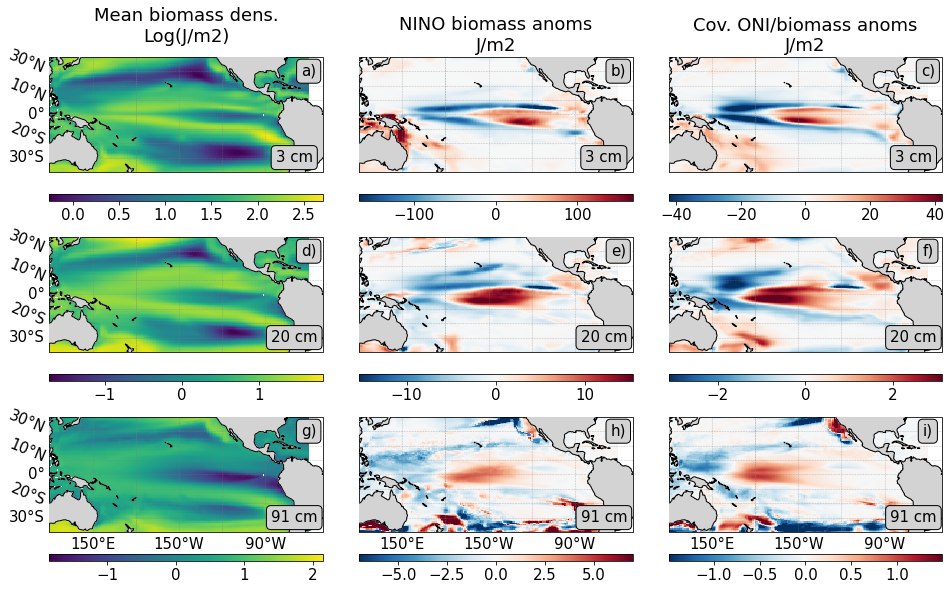
\includegraphics[scale=0.4]{figs/map_mean_anom_OND_97.png}	
	\caption{OND-NINO anomalies (left column) and covariance of fish biomass anomalies with the ONI index (right column) for small (upper line), intermediate (middle line) and large sizes (lower line). Black contours show the contours of mean fish biomass density (log-scale).}	
	\label{fig:mean_ond97_ape}
\end{figure}

In order to insure that the extreme El Nino composites give a robust view of fish biomass response to ENSO variability, covariance maps are computed between the monthly ONI index and the detrended fish biomass anomalies over the 1958-2018 period (right column of Fig\ref{fig:mean_ond97_ape}). The El Nino composites and the covariance maps are very similar, despite westward shifted anomalies and lower amplitudes for the covariance maps compared to the composites. These  differences are due to the fact that covariance analysis includes Central Pacific (i.e. Modoki) El Nino events (such as the 1986, 1991, 1994, 2002, 2004 and 2009 events) and La Nina events, whose signature is not opposite to Eastern Pacific events. Nevertheless, the general agreement between the covariance maps and the El Nino composites suggest that the focus on the three major events gives a general view of fish biomass response to ENSO.

Figure \ref{fig:profiles} shows the mean equatorial profiles for temperature, zonal velocity, low-trophic level concentration and fish-biomass (contour lines) and the composites of OND El Nino anomalies. Mean temperature shows a deep thermocline in the western Pacific and a shallow one in the east, which flattens during El Nino conditions, hence leading to a warming in the east and a cooling in the west. The structure of the Equatorial Undercurrent is well visible on the zonal velocity profile. It strongly weakens during El Nino conditions, while strong positive (i.e. eastward) anomalies occur near the surface. Low-trophic level concentrations are maximum in the top 50m of the eastern Pacific and decrease during El Nino conditions, due to the flattening of the thermocline, which is associated with a decrease in nutrient supply.

Right columns of Fig \ref{fig:profiles} show the equatorial profiles of fish biomass density for the three size-classes. On average, biomass in the western Pacific reaches $100m$, while in the eastern Pacific, it remains very close to the surface $25m$. The western biomass for small sizes is maximal close at the surface close to the dateline, while for intermediate and large sizes, the maximum occurs at $50m$ in the western Pacific (between 150 and 160\degree{}E)
During El Nino conditions, fish biomass shows an increase in the eastern Pacific (except very close to the surface) and a decrease in the west. However, the latter is not homogeneous on the vertical, since positive anomalies are located at around 50m in the east for intermediate and large sizes. These anomalies are induced by a tightening of the vertical habitat, due to the thermocline flattening, which in turn modifies the vertical distribution of fish biomass.

\begin{figure}[h!tp]
	\centering
	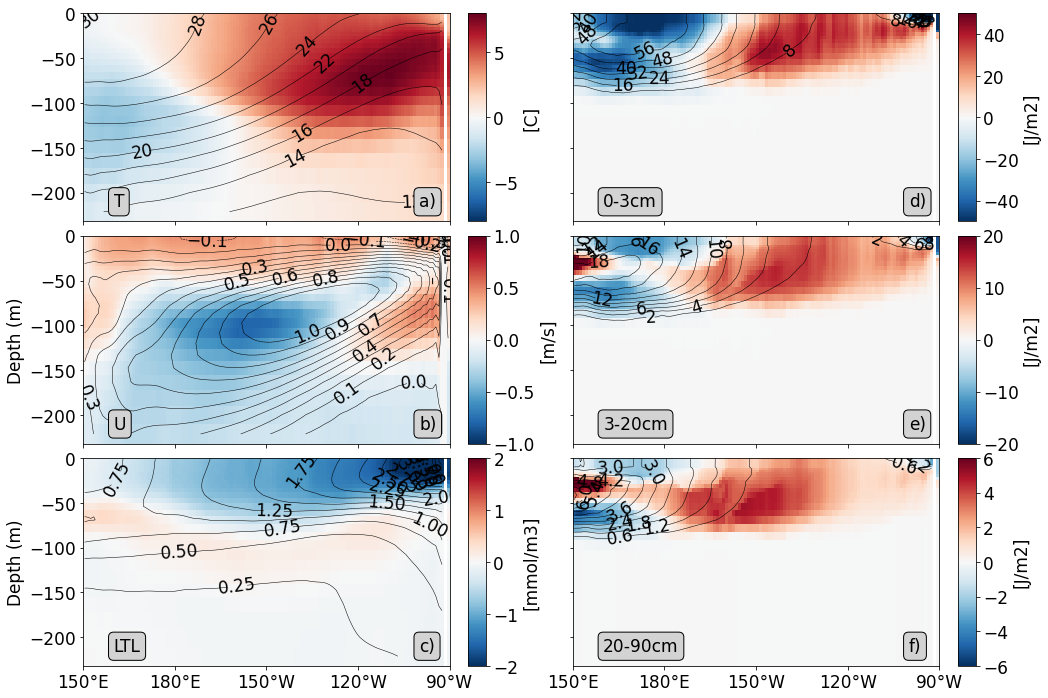
\includegraphics[scale=0.4]{figs/forage_mean_ond97.png}	
	\caption{Pacific equatorial profiles of temperature (a), zonal velocity (b), low-trophic concentration (c) and fish biomass (d for small, e for intermediate and f for large sizes). Mean are represented as black contour lines and El Nino anomalies are represented in colors.}	
	\label{fig:profiles}
\end{figure}

\subsection{Mechanisms and timing of the El Nino response}

In order to analyse the mechanisms and the timing of the fish biomass response to El Nino conditions, Hovmoller diagrams have been computed as follows. Monthly anomaly composites have been computed along the equatorial Pacific for the El Nino and subsequent years. 

Figures \ref{fig:hov_nemo_ape}a, \ref{fig:hov_nemo_ape}b, \ref{fig:hov_nemo_ape}c show the  Hovmüller diagrams of the temperature, chlorophyll and zonal currents anomalies averaged over the top 50m. In agreement with observations (not shown; see \cite{lengaigneOceanResponseMarch2002}), the warming signal associated with El Niño initiates in early spring (months 5 and 5) over the central and eastern equatorial Pacific, peaks by the end of the calendar year (months 10, 11, 12) in the eastern Pacific to quickly recede and switches La Niña conditions the following spring (month 16, Fig.\ref{fig:hov_nemo_ape}a). Simulated plankton concentration anomalies tend to mirror temperature anomalies, with a strong decline during El Niño and an enhanced bloom during La Niña (Figure \ref{fig:hov_nemo_ape}.b). 
The El Niño warming period is accompanied by strong surface eastward anomalous currents (Figure \ref{fig:hov_nemo_ape}c) promoted by anomalous westerly winds and contributing to central Pacific warming and eastward shift of the warm-pool towards the eastern equatorial Pacific. These current anomalies reverse during La Niña. 

\begin{figure}[h!tp]
	\centering
	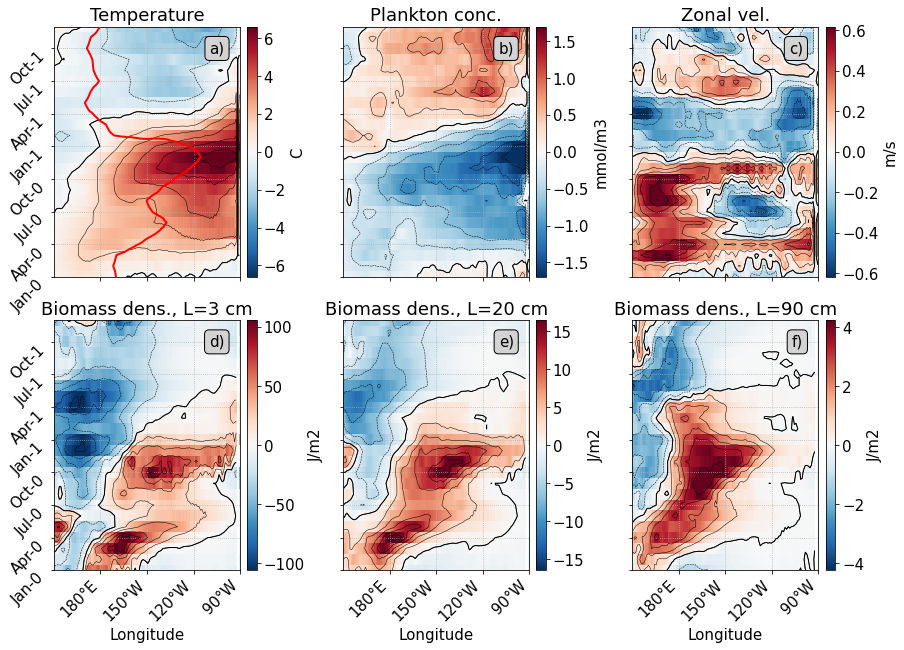
\includegraphics[scale=0.4]{plot_all_hovmoller_phys_oope.png}	
	\caption{Hovmoller diagrams of equatorial temperature (a), low-trophic level concentrations (b), zonal velocity (c) and fish biomass anomalies (3cm, 20cm and 90 cm in d, e, f, respectively).}	
	\label{fig:hov_nemo_ape}
\end{figure}

The same analysis is performed for epipelagic biomass for the three targeted size classes (Fig\ref{fig:hov_nemo_ape}d, Fig\ref{fig:hov_nemo_ape}e and Fig\ref{fig:hov_nemo_ape}f), which share some common features: positive biomass anomalies first appear near the dateline and propagate eastward towards the central Pacific until the end of spring (months 5 and 6). Another positive patch then develops in the central Pacific in fall and quickly recedes in winter. These positive anomalies in the central and eastern Pacific are associated with negative anomalies in the western Pacific. These negative anomalies persist after the El Nino demise and during the following La Nina event but remain restricted to the western Pacific. While sharing similarities, the response of larger epipelagic fishes is generally shifted westward compared to smaller ones, and the two consecutive increases in fish bish biomass are mixed-up for large sizes.

In order to determine the mechanisms behind the patterns of \ref{fig:hov_nemo_ape}, the same Hovmoller diagrams have been computed for different biological variables, such as the growth rate ($\gamma$ in equation \ref{eq:apecosm_trend}), the functional response and the predation mortality rates ($M$ in equation \ref{eq:apecosm_trend}). The same thing is also done for the right-hand side members of \ref{eq:apecosm_trend}, but the latter have been integrated over time, in order to extract the changes in fish biomass from the first month (month 1) to the last one (month = 24). The results are presented for each size class separately.

\subsection{3 cm}

\begin{figure}[h!tp]
	\centering
	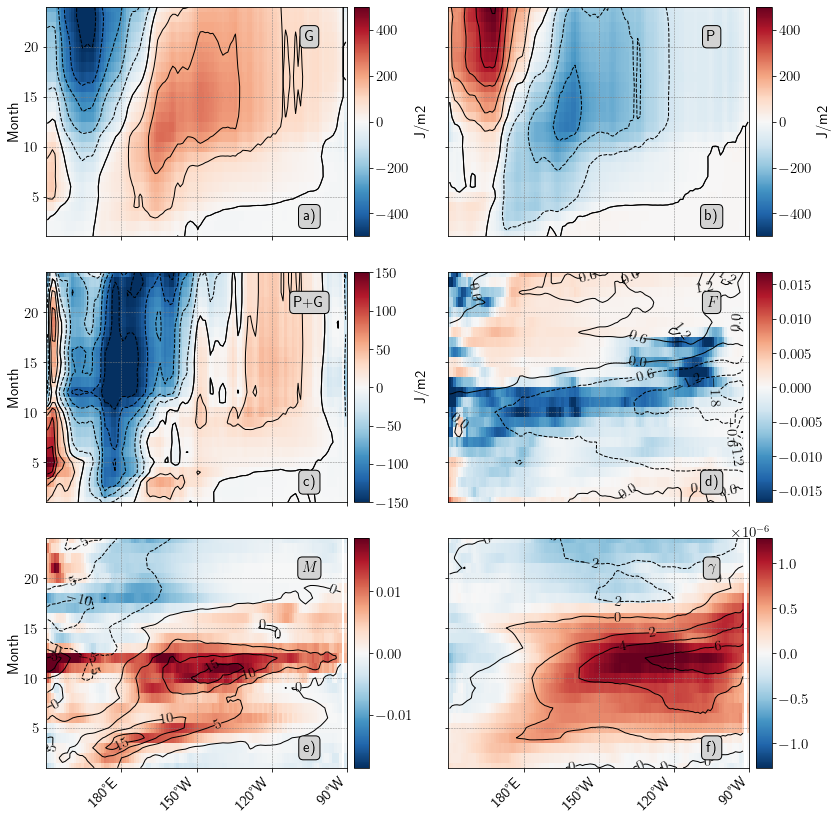
\includegraphics[scale=0.4]{figs/hov_compo_l_3.png}	
	\caption{Hovmoller diagrams of equatorial small fish biomass changes induced by growth (a), predation (b) and both contributions (c). Functional response anomalies (d, colors) and LTL concentration anomalies (d, contours). Predation mortality rates (e, colors) and intermediate fish biomass anomalies (e, contours). Growth rate (f, colors) and temperature anomalies (f, contours)}	
	\label{fig:hov_ape_trends_3}
\end{figure}

Predation and growth show opposite contributions to changes in small fish biomass (Fig.\ref{fig:hov_ape_trends_3}a and Fig.\ref{fig:hov_ape_trends_3}.b), which are around 3 times larger than the biomass anomalies (Fig. \ref{fig:hov_nemo_ape}d), implying that at first order these anomalies balance each other. At month 5, growth induces a biomass increase in the central Pacific (between dateline and 150\degree{}W), while predation induces a decrease. Starting in month 10, these relative contributions to fish biomass anomalies extend to the east, and opposite contributions appear in the western Pacific. Interestingly, the anomalies induced by growth are westward shifted and start later than the temperature increase induced by the onset of El Nino conditions. Growth rates changes closely follow changes in temperature, while predation mortality rates closely follow changes in larger fish biomass (not shown). The functional response, which depends both on temperature and food density, show negative anomalies which are consistent with the reduction of low-trophic concentrations, hence suggesting a dominance of food density on the functional response.

The pattern obtained by summing these two contributions (Fig.\ref{fig:hov_ape_trends_3}.c) is a negative anomaly centered around the dateline and extending from months 1 to 24, with the strongest anomalies in early 1998, and positive anomalies that appears at month 10 at 120\degree{}W. These sole biological contributions, however, do not explicitely looks like the biomass anomalies depicted on Fig.\ref{fig:hov_nemo_ape}d, and advection and diffusion processes must be considered as well. Although their contributions seem a bit more noisy, it somehow counteracts the changes of fish biomass induced by growth and predation. Especially, it induces negative anomalies in the eastern Pacific (month 12 and 120\degree{}W), which compensate the positive ones induced by predation and growth. 

Therefore, the response of small fish biomass to El Nino events is a strong biological response through predation and growth, which both compensate each other . The remaining, in turn, is in balance with advection and diffusion processes.

\subsection{20 cm}

Regarding intermediate size-classes, changes in biomass induced by growth and predation are of the same order of magnitudes as changes in fish biomass. Changes induced by growth processes strongly ressemble the ones obtained for small sizes, with an increase in fish biomass in that starts at 180\degree{}E at month 2, and which propagates eastward. At month 10, the positive anomalies peak at 150\degree{}W, while negative anomalies take place in the western Pacific (170\degre{}E). Contrary to what occurred for small sizes, changes induced by predation mortality do not mirror changes induced by growth. Indeed, predation mortality induce mostly a reduction of intermediate fish biomass, which starts at month 5 in the western Pacific and propagates eastward, to reach its maximum at 170\degree{}W and at month 10. The changes induced by the combination of both processes resembles the one obtained for small sizes but are westward shifted. As for small sizes, the sole biological processes do not explain do not explain the fish biomass anomalies shown in Fig.\ref{fig:hov_nemo_ape}e, and the contributions of advection and diffusion need to be considered. They account for the two initial fish biomass increases that starts in month 3 at 180\degree{}E and in month 10 at 150\degree{}W. The comparison of active and passive velocities suggest that passive movements (i.e. advection by the ocean currents) dominate, with ocean current anomalies greater than active velocity anomalies by a factor of $\approx\ 20$.

The functional response of intermediate show the same pattern than the growth rate, contrary to small sizes, for which the anomalies are opposite in sign. This indicates that for intermediate sizes, growth rate and functional response are controlled by the same processes. In this case, it can be due to both an increase in food availability, provided by the increase of small sizes biomass, and the warmer temperatures associated with El Nino conditions. Predation mortality rates, without any surprise, show positive anomalies where large fish biomasss increase.

\begin{figure}[htp]
	\centering
	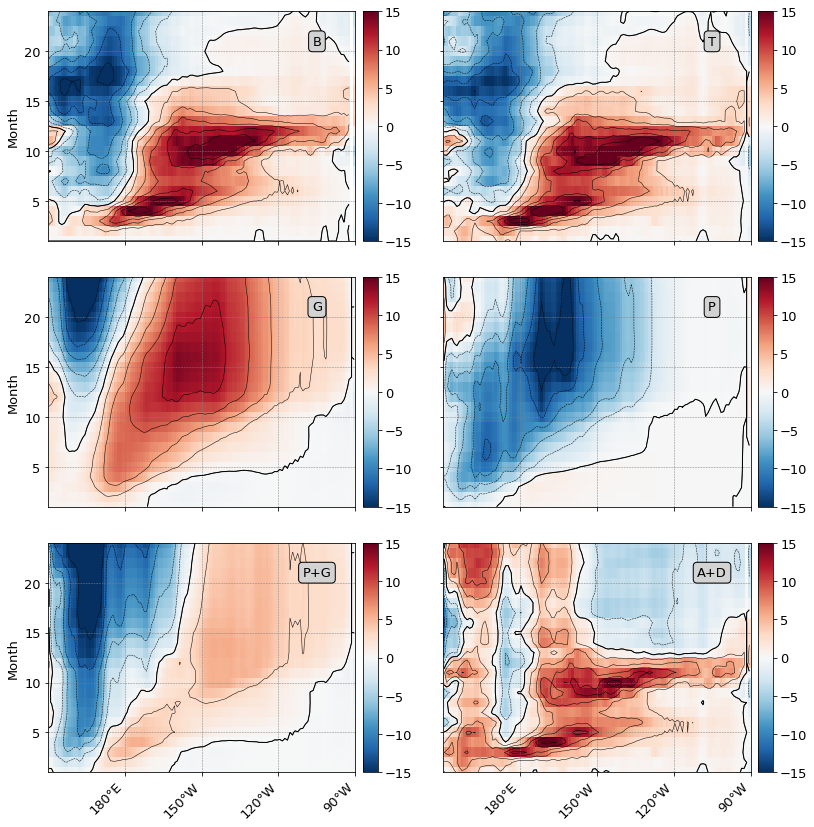
\includegraphics[scale=0.4]{figs/hov_compo_l_20.png}	
	\caption{Hovmoller diagrams of equatorial intermediate fish biomass anomalies induced by predation mortality (P, first line), growth (G, second line), growth + predation (P+G, third line) and movements (advection and diffusion, A+D, bottom line)}	
	\label{fig:hov_ape_trends_20}
\end{figure}

\subsubsection{90 cm}

For large sizes, changes in fish biomass is dominated by advection/diffusion processes, while predation and growth have barely no impact. The possible reason is that as size increases, biological processes tend to be slower (\warn{is it true?}). Therefore, the biological response of large sizes to interannual events don't have necessary time to set-up. As a consequence, the interannual variability is solely driven by fish movements.



They are both associated with positive anomalies west of the dateline, and negative anomalies between the dateline and 150W. However, these anomalies do not seem to change much between 1997-01 and 1998-12 and therefore cannot explain the large fish biomass anomalies depicted in Fig.\ref{fig:hov_nemo_ape}f. On the other hand, the fish biomass anomalies induced by advection and diffusion perfectly match the simulated fish biomass anomalies. \warn(Specify if diffusion/advection, specify if active or passive). Therefore, on interannual time-scales, fish biomass for large sizes is not driven by biological processes but by physical ones.

\begin{figure}[h!tp]
	\centering
	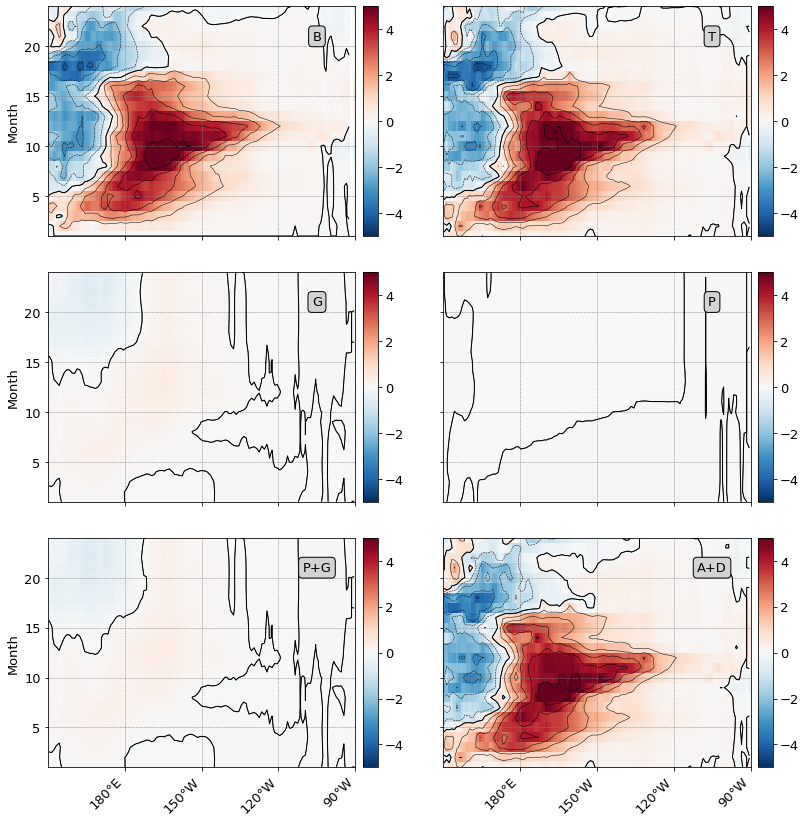
\includegraphics[scale=0.4]{figs/hov_compo_l_90.png}	
	\caption{Hovmoller diagrams of equatorial large fish biomass anomalies induced by predation mortality (P, first line), growth (G, second line), growth + predation (P+G, third line) and movements (advection and diffusion, A+D, bottom line)}	
	\label{fig:hov_ape_trends_90}
\end{figure}



%The patterns of the functional response and growth rates are very different for small sizes (figures YYY.a and YYY.d). The former shows negative anomalies on the central Pacific during the onset of El Nino conditions, presumably due to the concomitant reduction of plankton concentration (figure YYY.b). Interestingly, no anomalies are found in the eastern basin, due to compensating effects of warming temperatures and reduced plankton concentrations. The growth rate shows a pattern that is very similar to the temperature anomalies (Fig. XXX.a), indicating the dominance of temperature on the growth rate. The mortality rate (Fig. YYY.g) shows a pattern that is consistent with the increased biomass of intermediate epipelagics (XXX.b), which predate on small ones.  Besides, growth rate anomalies superimpose well on the small biomass anomalies (black contours in Fig. YYY.d), hence suggesting that the increased biomass during the El Nino conditions is triggered by enhanced growth associated with warmer temperature, despite a dampening effect of increased mortality rates.
%For intermediate sizes, the functional response and the growth rate show very similar anomalies, hence suggesting that they both are driven by the same factors. Both show positive anomalies during the onset of El Nino between 200E and 250E, presumably induced by the temperature warming that favours both the growth and search rates. Then negative anomalies occur, which are westward shifted relative to the positive ones. These negative anomalies are likely induced by the cooling associated with the La Nina conditions reinforced by the reduced small fish biomass that appears near 200E, as shown in Fig. XXX.d. Mortality rates anomalies are consistent with the increase of large fish biomass (Fig. XXX.f). Comparing the different fields, we can suggest that the increased fish biomass that appears on the central Pacific in early 1997 is first dominated by advective processes, which returns a similar pattern (fig YYY.k). Then, during the El Nino peak, the increased biomass of intermediate fish is driven by both an increased growth rate and an increased functional response, which are induced by warmer temperatures and more food available (more small epipelagic fishes, Fig. XXX.d).

%\subsection{Generalisation}
%
%In order to see if ecosystem response to the 97 El Nino event is representative, the covariance between fish biomass anomalies and the ONI index have been computed, following the methodology described in section \ref{sec:cov}. The maps are presented in Fig\ref{fig:ape_cov}.
%
%\begin{figure}
%	\centering
%	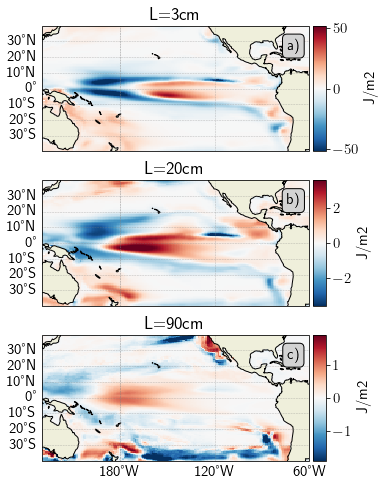
\includegraphics[scale=0.6]{figs/fig7.png}	
%	\caption{Covariance maps between the ONI index and the vertically integrated fish biomass anomalies for small (a), intermediate (b) and large (c) sizes.}	
%	\label{fig:ape_cov}
%\end{figure}
%
%The covariance patterns are very similar to the biomass anomalies depicted in Fig\ref{fig:mean_ond97_ape}, therefore suggesting that the mechanisms described in the above  apply to the general case. However, we note that the covariance patterns are westward shifted compared to the fish biomass anomalies. 
%
%This westward shift might be explained by the fact that when performing covariance anomalies, different El Nino events (Easter Pacific El Nino, Central Pacific El Nino) and La Nina events are considered, which ultimately impacts the global view of fish biomass response to ENSO variability.


%In this section, the interannual response of epipelagics to ENSO variability is investigated using covariance analysis. The left panels of Figure 3. show the yearly mean vertically integrated fish biomass over the entire simulation for the three different size classes. For small sizes (Figure 3a), the fish biomass is concentrated at around 10° S and 10 ° N in the central Pacific and close to the equator in the western Pacific. High biomass concentration is also found east of 90° W, off the coasts of Chile. As size increases, the equatorial "blue spot" extends meridionnally and to the west. This pattern is mostly driven by the active and passive advection of fishes in the Apecosm model (REF). Without advection, the biomass will be concentrated at the equator, where the plankton concentration is the maximum.
%
%Covariance maps between vertically integrated fish biomass and the winter ONI index are shown in the right panels of Figure 3. Small epipelagics show negative anomalies in the Western Equatorial Pacific and positive anomalies in the Central Equatorial Pacific. This pattern can be interpreted as an eastern displacement of the mean biomass in the Western Pacific. Similar dipolar patterns are also obtained for intermediate and large sizes, but the anomalies westward shifted as size increases. This can be interpreted, as for small sizes, by a westward shift of fish biomass during positive El Niño phases. The same results have been obtained when the covariance analysis is performed on monthly anomalies (not shown).